\chapter{Diseño e implementación} % Main chapter title

\label{Chapter3} % Change X to a consecutive number; for referencing this chapter elsewhere, use \ref{ChapterX}

En este capítulo se describen el diseño e implementación del sistema desarrollado, tanto del dispositivo en general como los diferentes módulos de firmware que lo componen. También se presenta la interfaz de usuario y el protocolo de comunicación empleado entre el microcontrolador y la aplicación de escritorio.

\definecolor{mygreen}{rgb}{0,0.6,0}
\definecolor{mygray}{rgb}{0.5,0.5,0.5}
\definecolor{mymauve}{rgb}{0.58,0,0.82}

%%%%%%%%%%%%%%%%%%%%%%%%%%%%%%%%%%%%%%%%%%%%%%%%%%%%%%%%%%%%%%%%%%%%%%%%%%%%%
% parámetros para configurar el formato del código en los entornos lstlisting
%%%%%%%%%%%%%%%%%%%%%%%%%%%%%%%%%%%%%%%%%%%%%%%%%%%%%%%%%%%%%%%%%%%%%%%%%%%%%
\lstset{ %
  backgroundcolor=\color{white},   % choose the background color; you must add \usepackage{color} or \usepackage{xcolor}
  basicstyle=\footnotesize,        % the size of the fonts that are used for the code
  breakatwhitespace=false,         % sets if automatic breaks should only happen at whitespace
  breaklines=true,                 % sets automatic line breaking
  captionpos=b,                    % sets the caption-position to bottom
  commentstyle=\color{mygreen},    % comment style
  deletekeywords={...},            % if you want to delete keywords from the given language
  %escapeinside={\%*}{*)},          % if you want to add LaTeX within your code
  %extendedchars=true,              % lets you use non-ASCII characters; for 8-bits encodings only, does not work with UTF-8
  %frame=single,	                % adds a frame around the code
  keepspaces=true,                 % keeps spaces in text, useful for keeping indentation of code (possibly needs columns=flexible)
  keywordstyle=\color{blue},       % keyword style
  language=[ANSI]C,                % the language of the code
  %otherkeywords={*,...},           % if you want to add more keywords to the set
  numbers=left,                    % where to put the line-numbers; possible values are (none, left, right)
  numbersep=5pt,                   % how far the line-numbers are from the code
  numberstyle=\tiny\color{mygray}, % the style that is used for the line-numbers
  rulecolor=\color{black},         % if not set, the frame-color may be changed on line-breaks within not-black text (e.g. comments (green here))
  showspaces=false,                % show spaces everywhere adding particular underscores; it overrides 'showstringspaces'
  showstringspaces=false,          % underline spaces within strings only
  showtabs=false,                  % show tabs within strings adding particular underscores
  stepnumber=1,                    % the step between two line-numbers. If it's 1, each line will be numbered
  stringstyle=\color{mymauve},     % string literal style
  tabsize=2,	                   % sets default tabsize to 2 spaces
  title=\lstname,                  % show the filename of files included with \lstinputlisting; also try caption instead of title
  morecomment=[s]{/*}{*/}
}


%----------------------------------------------------------------------------------------
%	SECTION 1
%----------------------------------------------------------------------------------------
\section{Arquitectura general del sistema}

El sistema desarrollado constituye un dispensador automático de alimento seco para gatos, capaz de operar de forma autónoma sin dependencia de una conexión a Internet. El dispositivo gestiona la entrega de alimento en horarios programados, monitorea el peso del tanque de almacenamiento y del plato de consumo. Esta información se comunica al usuario a través de una aplicación de escritorio mediante Bluetooth.

El componente central del sistema es el microcontrolador STM32F446RE, que actúa como unidad de procesamiento principal. Este componente coordina la lectura de los sensores de pesaje, controla el motor de dispensado y administra la comunicación con los módulos periféricos. La figura \ref{fig:bloques} presenta el diagrama en bloques del sistema, donde se distinguen tres bloques funcionales principales: sensado, control y comunicación con el usuario.

\begin{figure}[H]
    \centering
    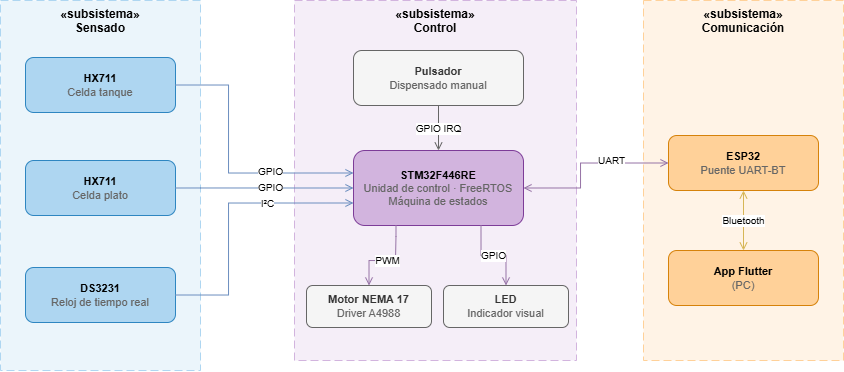
\includegraphics[width=0.85\textwidth]{./Figures/diagrama_bloques.png}
    \caption{Diagrama en bloques del sistema.}
    \label{fig:bloques}
\end{figure}

El bloque de sensado comprende dos módulos HX711 conectados a sus respectivas celdas de carga: uno ubicado bajo el tanque de almacenamiento y otro bajo el plato. A estos se suma el módulo DS3231, que provee la referencia temporal necesaria para la gestión autónoma de los horarios de dispensado.

El bloque de control concentra toda la lógica de la aplicación en el microcontrolador, e incorpora también el motor paso a paso NEMA 17 con su driver A4988, el pulsador de dispensado manual y el LED de estado del sistema. 

El bloque de comunicación con el usuario está compuesto por el módulo ESP32, que opera como puente entre el microcontrolador y la aplicación de escritorio desarrollada en Flutter, a través de Bluetooth Classic.


\section{Arquitectura de hardware}

En esta sección se describe la interconexión entre los componentes electrónicos que conforman el sistema, junto con el análisis de potencia necesario para garantizar su correcto funcionamiento.

\subsection{Alimentación y microcontrolador}

En primera instancia, se debe resolver el requerimiento de alimentación del sistema. A diferencia de soluciones portátiles basadas en batería, el presente trabajo utiliza una fuente de alimentación de 12 V de corriente alterna como fuente de energía principal. Esta decisión se fundamenta en el elevado consumo del motor paso a paso NEMA 17 con su driver A4988, que en condiciones de máxima carga puede demandar hasta 2 A, lo que hace inviable el uso de una batería para una operación continua y prolongada.

Dado que la totalidad de los componentes del sistema opera a una tensión nominal de 5 V, se incorpora un regulador de voltaje reductor (\textit{step-down}) basado en el integrado LM2596S \cite{LM2596S}, capaz de aceptar tensiones de entrada de hasta 35 V y entregar una corriente máxima de 3 A con tensión de salida ajustable. La figura \ref{fig:step_down} muestra el módulo comercial utilizado, y la figura~\ref{fig:conexion_alimentacion} ilustra su conexión con el microcontrolador.

\begin{figure}[H]
    \centering
    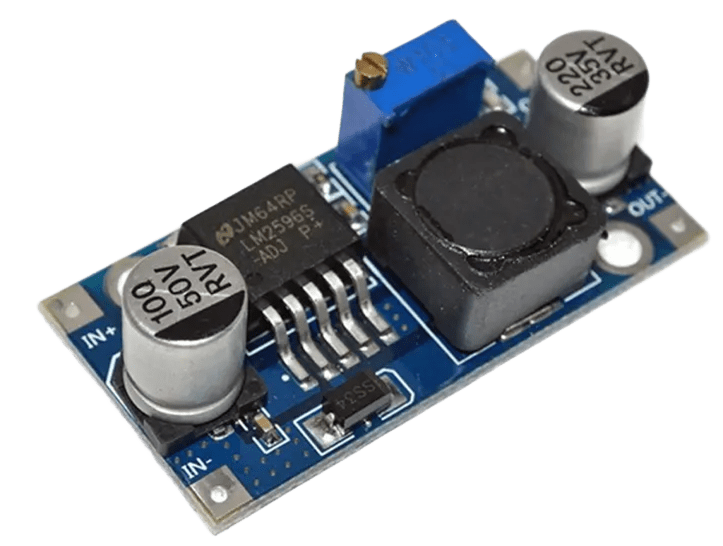
\includegraphics[width=4cm, height=4cm]{./Figures/step_down.png}
    \caption{Módulo regulador de voltaje reductor basado en el LM2596S.\protect\footnotemark}
    \label{fig:step_down}
\end{figure}
\footnotetext{Imagen del módulo comercial LM2596S.}

\begin{figure}[H]
    \centering
    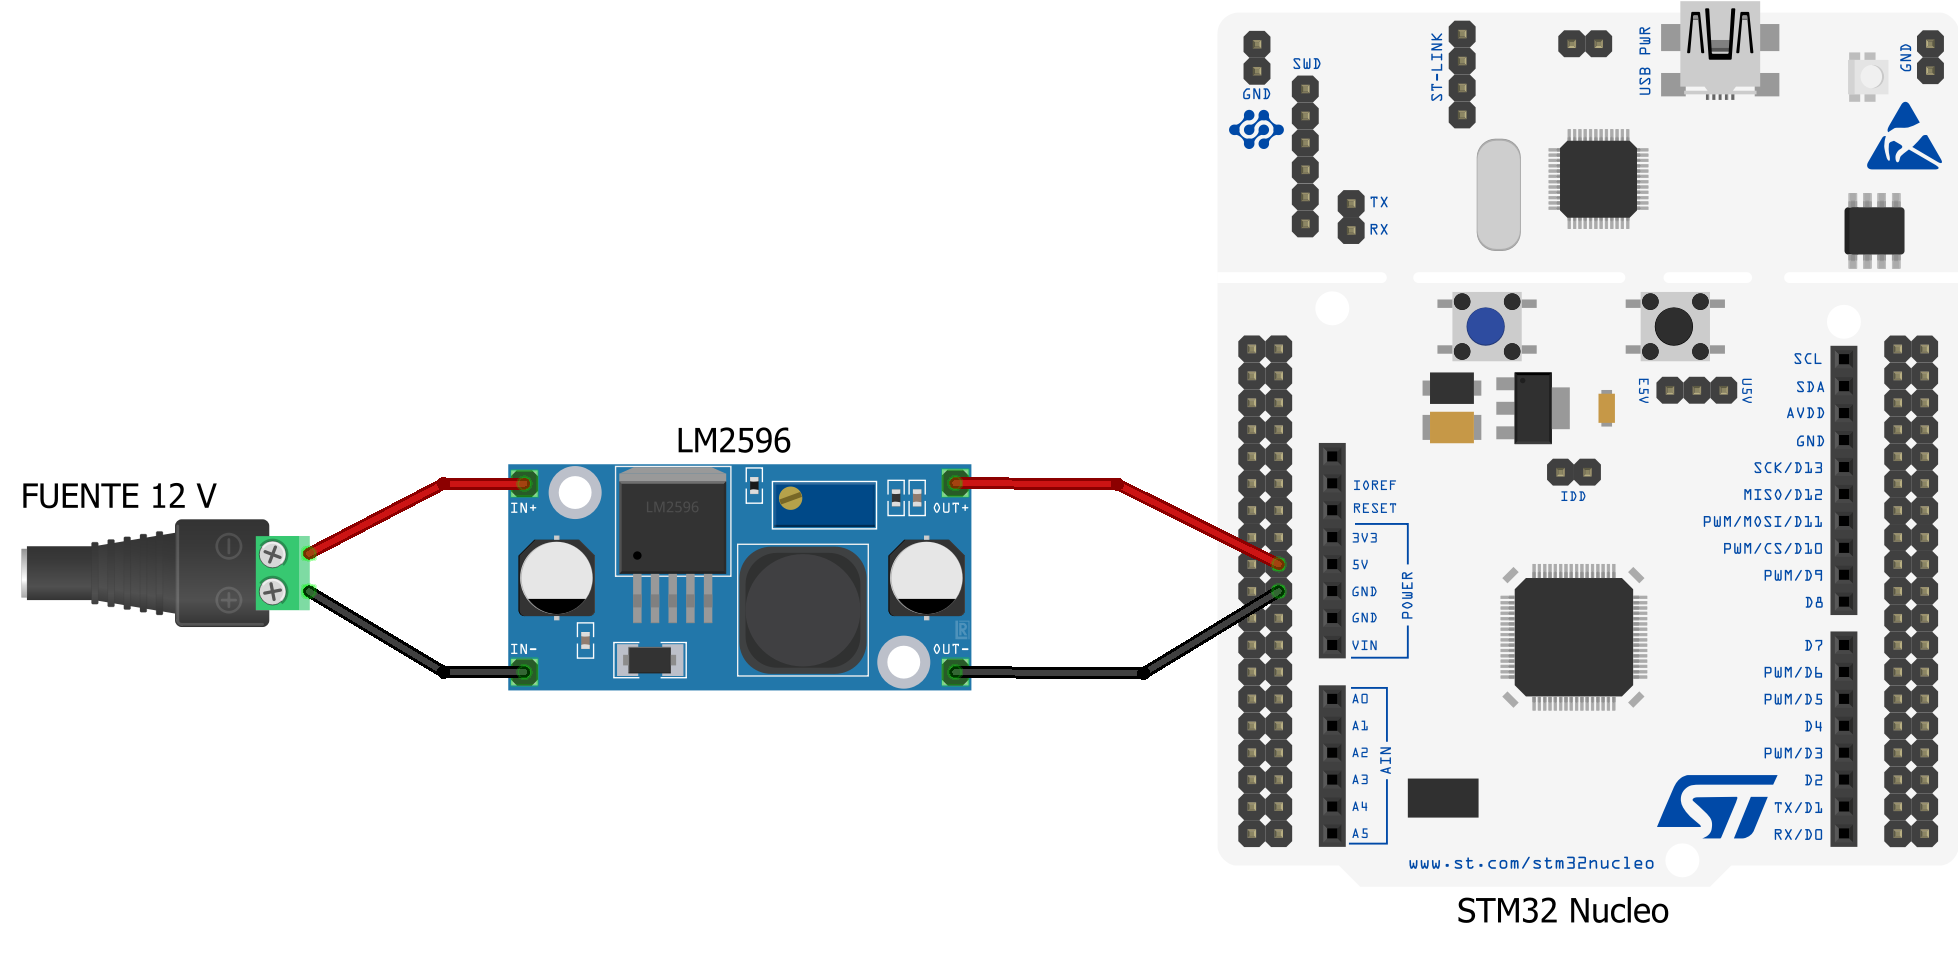
\includegraphics[width=0.75\textwidth]{./Figures/conexion_alimentacion.png}
    \caption{Interconexión entre la fuente de alimentación y el microcontrolador.}
    \label{fig:conexion_alimentacion}
\end{figure}


\subsection{Interconexión de componentes}
Una vez presentados los componentes del sistema en el capítulo anterior, se describe a continuación cómo se interconectan entre sí. Todos los módulos operan a una tensión nominal de 5 V, por lo que comparten la misma fuente de alimentación. 

El microcontrolador STM32F446RE se comunica con los dos módulos HX711 mediante señales digitales GPIO. Cada módulo HX711 emplea una interfaz de dos cables: uno de reloj (CLK) y uno de datos (DATA), conectados a pines GPIO del microcontrolador configurados como salida y entrada respectivamente. El módulo DS3231 se conecta al microcontrolador a través del bus I\textsuperscript{2}C, utilizando las líneas SCL y SDA del periférico I2C1, configurado a 400 kHz. El módulo ESP32 se conecta mediante el periférico UART4, configurado a 115.200 baudios con formato 8N1. El pulsador de dispensado manual se conecta a un pin configurado como entrada con interrupción externa (EXTI), con un tiempo de antirrebote de 200 ms implementado por software. El LED de estado se conecta a una salida GPIO de propósito general. La figura~\ref{fig:conexion_perifericos} muestra el esquema de estas conexiones.

\begin{figure}[H]
    \centering
    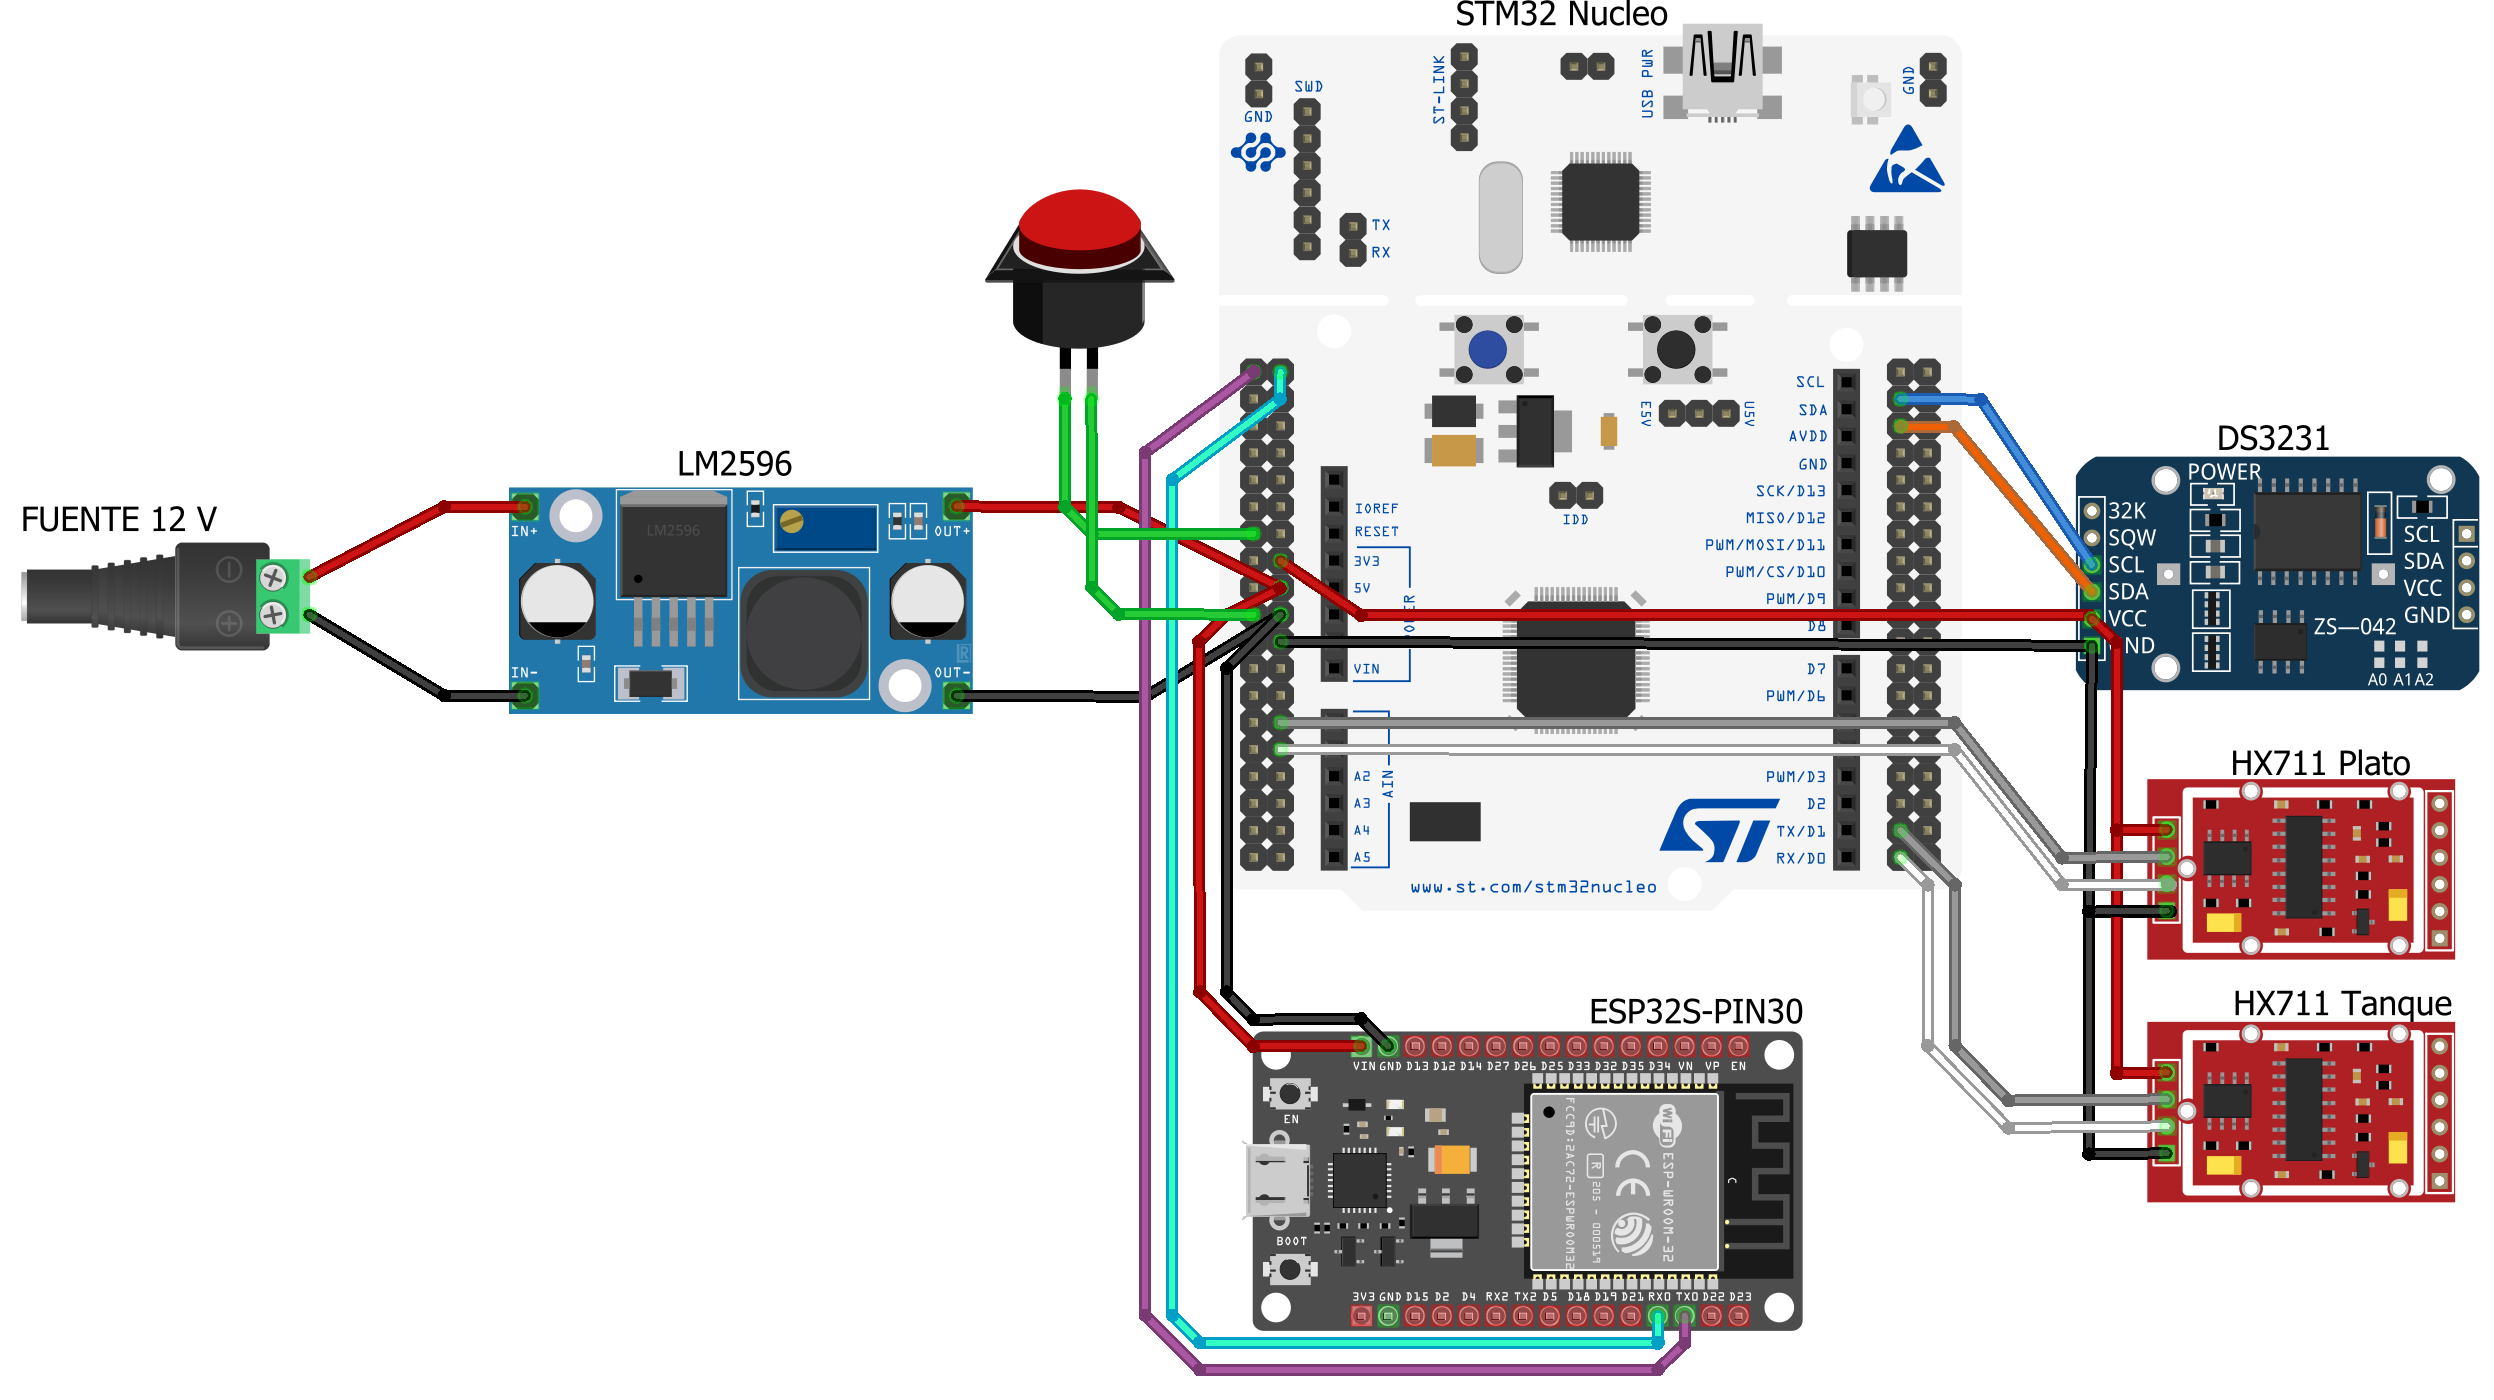
\includegraphics[width=0.85\textwidth]{./Figures/conexion_perifericos.png}
    \caption{Interconexión entre el microcontrolador y sus periféricos.}
    \label{fig:conexion_perifericos}
\end{figure}

El motor paso a paso NEMA 17 se controla a través del driver A4988, que recibe tres señales digitales provenientes del microcontrolador: la señal STEP, generada por el canal 3 del temporizador TIM2 en modo PWM sobre el pin PB10; la señal DIR, que define el sentido de giro; y la señal ENABLE, que habilita o deshabilita el driver. Las señales DIR y ENABLE se manejan como salidas GPIO simples. La figura~\ref{fig:conexion_motor} ilustra el esquema de conexión entre el microcontrolador, el driver y el motor.

\begin{figure}[H]
    \centering
    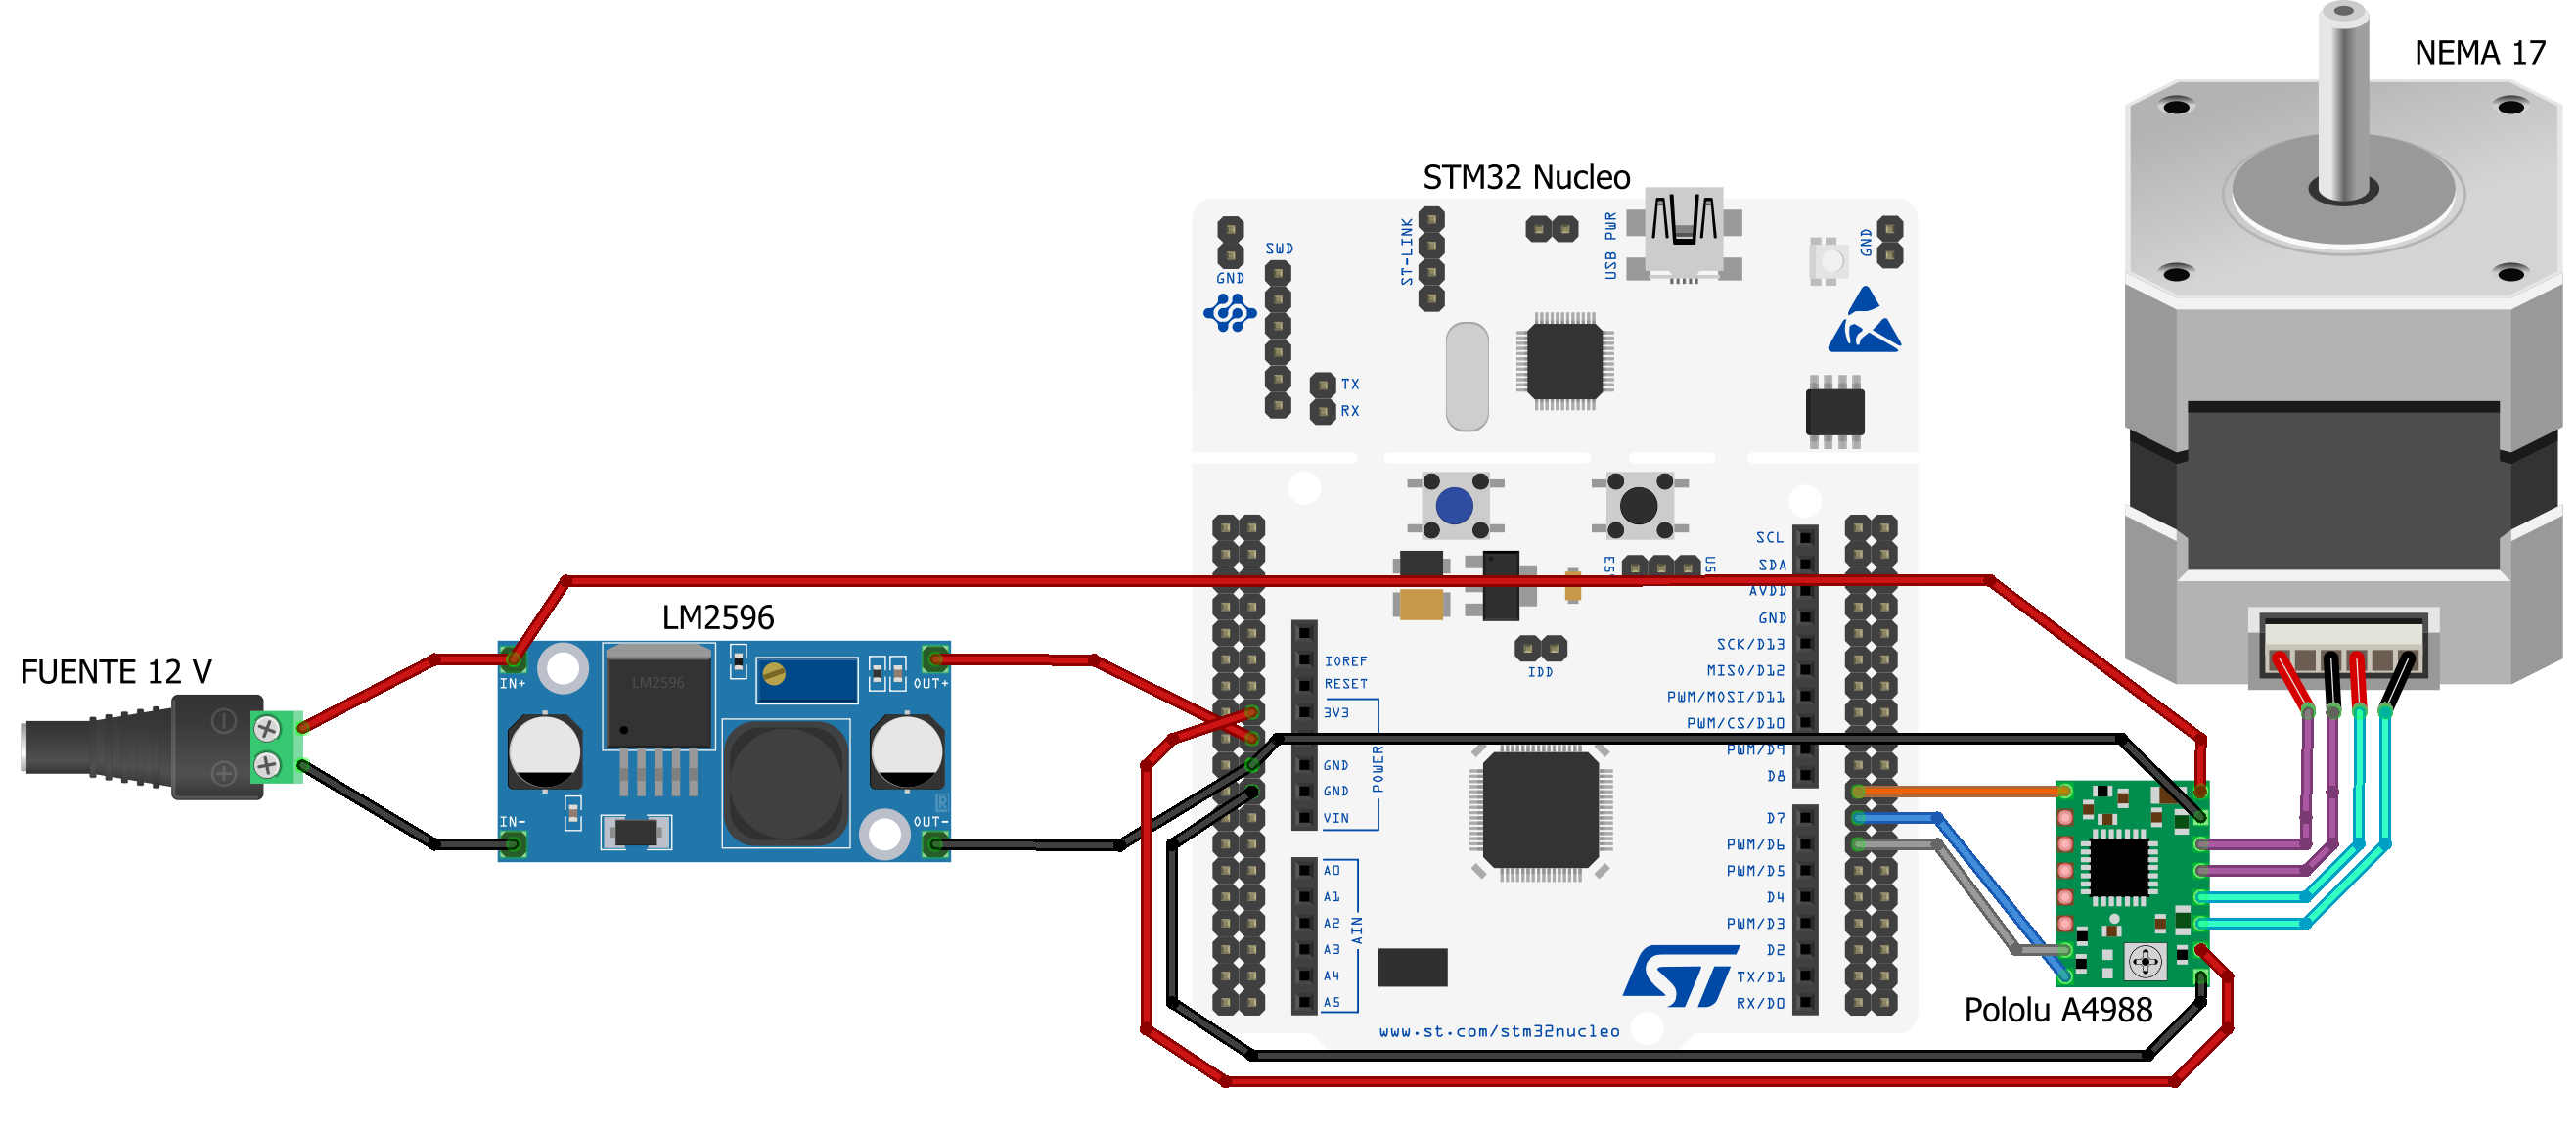
\includegraphics[width=0.85\textwidth]{./Figures/conexion_motor.png}
    \caption{Interconexión entre el microcontrolador, el driver A4988 y el motor NEMA 17.}
    \label{fig:conexion_motor}
\end{figure}


\subsection{Análisis de potencia}

El prototipo desarrollado requiere una fuente de alimentación capaz de proveer la corriente suficiente para todos los componentes del sistema de forma simultánea. La tabla~\ref{tab:potencia} resume el consumo máximo de cada componente según las hojas de datos de sus fabricantes.

\begin{table}[H]
\centering
\caption{Consumo máximo de cada componente del sistema.}
\label{tab:potencia}
\begin{tabular}{lcc}
\toprule
\textbf{Componente} & \textbf{Tensión (V)} & \textbf{Corriente máxima (mA)} \\
\midrule
STM32F446RE           & 5  & 36   \\
HX711 (×2)            & 5  & 3    \\
DS3231                & 5  & 1    \\
Driver A4988          & 5  & 10   \\
Motor NEMA 17         & 12 & 1700 \\
ESP32                 & 5  & 130  \\
LED de estado         & 5  & 20   \\
\bottomrule
\end{tabular}
\end{table}

Del análisis de la tabla se concluye que el componente de mayor consumo es el motor paso a paso NEMA 17, que opera a 12 V y puede demandar hasta 1,7 A por fase en condiciones de máxima carga. El resto de los componentes opera a 5 V con un consumo total aproximado de 200 mA. Estos valores justifican la elección de una fuente de alimentación de 12 V y el módulo regulador LM2596S, cuya corriente máxima de salida de 3 A provee el margen necesario para una operación confiable del sistema.


\section{Arquitectura de software}

En esta sección se describe la organización del firmware desarrollado para el microcontrolador STM32F446RE y la lógica de control que gobierna el comportamiento del sistema.

\subsection{Desarrollo del firmware}

Para implementar la lógica del trabajo, se desarrollaron módulos de software de forma independiente, con el propósito de que su desarrollo fuera autónomo y para facilitar su integración. La figura~\ref{fig:software_bloques} muestra el diagrama en bloques que representa los subsistemas que conforman el firmware.

\begin{figure}[H]
    \centering
    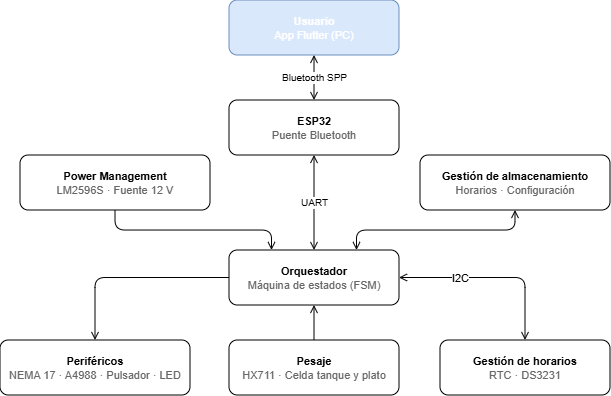
\includegraphics[width=0.52\textwidth]{./Figures/diagrama_software.png}
    \caption{Diagrama en bloques de subsistemas de software.}
    \label{fig:software_bloques}
\end{figure}

El módulo central del sistema es el orquestador, cuya función es inicializar todos los periféricos necesarios y luego gestionar la lógica de control a través de una máquina de estados. Para ello se utilizó FreeRTOS \cite{freertos_ref}, con dos tareas principales: una encargada del control del dispensado y otra dedicada a la comunicación con el usuario.

\subsection{Módulo orquestador}

El módulo orquestador gestiona el ciclo completo de operación del dispensador mediante una máquina de estados finita. La figura~\ref{fig:estados} presenta el diagrama de estados del sistema.

\begin{figure}[H]
    \centering
    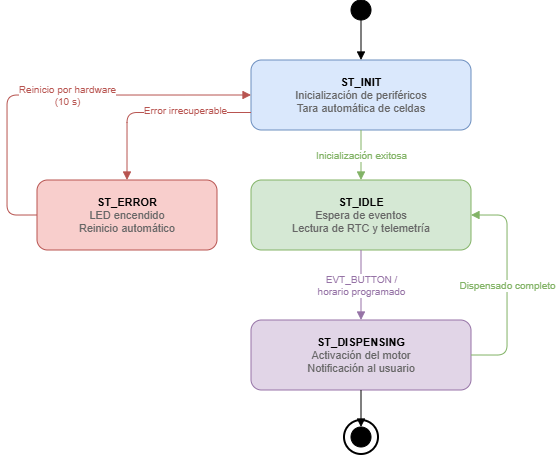
\includegraphics[width=0.52\textwidth]{./Figures/diagrama_estados.png}
    \caption{Diagrama de estados del dispensador.}
    \label{fig:estados}
\end{figure}

El sistema transmite dos tipos de mensajes hacia la aplicación. El primero es un mensaje de telemetría enviado cada 1 segundo que incluye el peso del tanque y el peso del plato, con la fecha y la hora provistas por el módulo DS3231. El segundo se emite al completarse un ciclo de dispensado e informa la cantidad dispensada, el origen del evento y la hora en que ocurrió. Desde la aplicación, el usuario puede enviar comandos para solicitar un dispensado manual, ejecutar la tara de las celdas de carga o actualizar los horarios programados.


\subsection{Módulo de comunicación}

El módulo de comunicación gestiona el intercambio de información entre el microcontrolador y la aplicación de escritorio a través del módulo ESP32. La comunicación es bidireccional y se estructura en dos tipos de mensajes: los mensajes salientes, que el sistema envía hacia la aplicación, y los comandos entrantes, que la aplicación envía hacia el sistema. Todos los mensajes se estructuran en formato \texttt{JSON} \cite{JSON}, lo que permite una integración sencilla con la aplicación de escritorio. La figura~\ref{fig:arquitectura_comm} ilustra la arquitectura de comunicación del sistema junto con los mensajes intercambiados.

\begin{figure}[H]
    \centering
    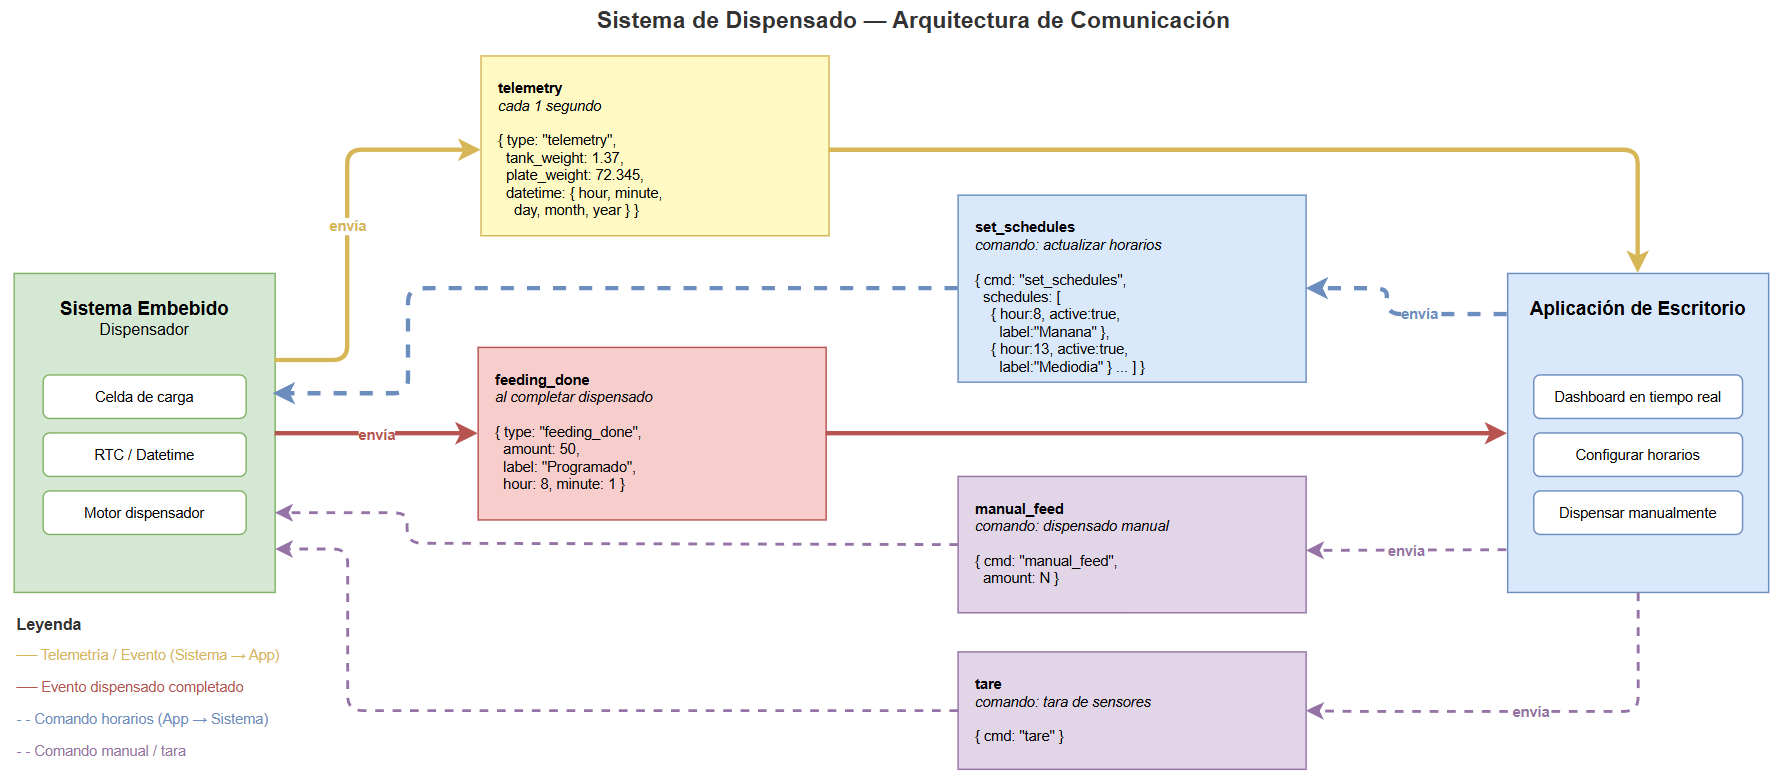
\includegraphics[width=0.95\textwidth]{./Figures/dispensador_arquitectura.png}
    \caption{Arquitectura de comunicación del sistema de dispensado.}
    \label{fig:arquitectura_comm}
\end{figure}

Entre los mensajes salientes se destaca el mensaje de telemetría, que se transmite cada 1 segundo e incluye el peso del tanque de almacenamiento, 
el peso del plato y la fecha y hora provistas por el módulo DS3231. Al completarse un ciclo de dispensado, el sistema envía un mensaje de evento 
que indica la cantidad dispensada, la etiqueta del horario y la hora en que ocurrió. Entre los comandos entrantes, la aplicación puede solicitar 
un dispensado manual, ejecutar la tara de las celdas de carga o actualizar los horarios programados.

\subsection{Interfaz de usuario}

La interfaz de usuario se implementó como una aplicación de escritorio desarrollada en Flutter, que corre sobre el sistema operativo Windows y 
se comunica con el sistema mediante Bluetooth Classic. La aplicación permite al usuario visualizar en tiempo real el peso del tanque de 
almacenamiento y del plato de consumo, consultar el historial de dispensados, configurar los horarios programados y ejecutar un dispensado 
manual o una tara de las celdas de carga. La figura~\ref{fig:app_flutter} muestra la interfaz principal de la aplicación.

\begin{figure}[H]
    \centering
    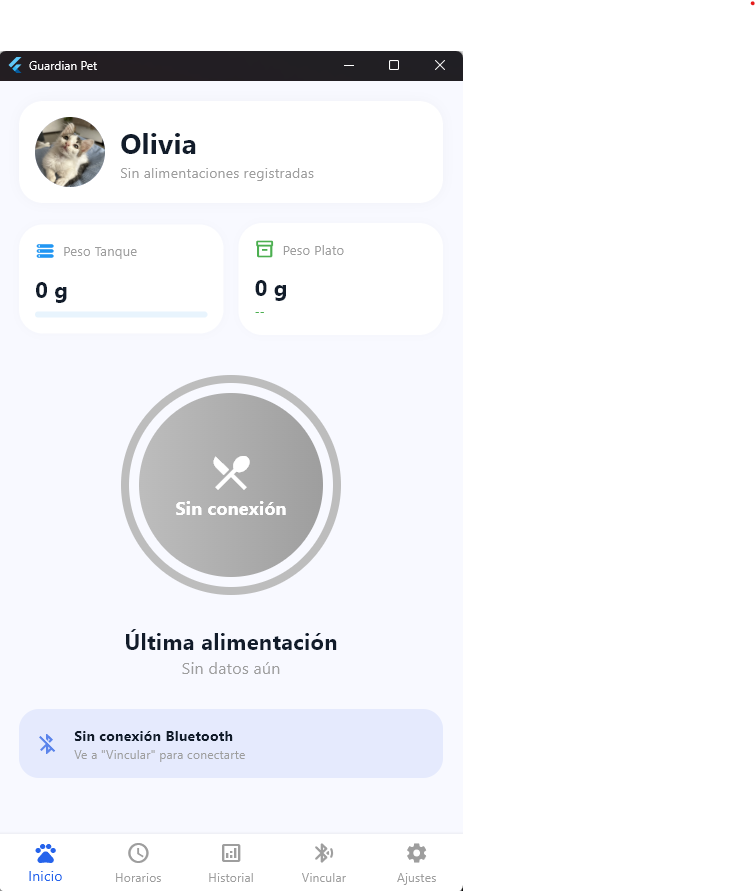
\includegraphics[
        width=0.45\textwidth,
        trim={0cm 0cm 6cm 0cm},
        clip
    ]{./Figures/app_flutter.png}
    \caption{Interfaz principal de la aplicación de escritorio 
    desarrollada en Flutter.}
    \label{fig:app_flutter}
\end{figure}